\section{Tests and Results}

\subsection{A first comparison}
For the performance evaluation, four versions of the MapReduce implementation were considered: 
\texttt{Hadoop-noimc}\footnote{IMC stands for \textit{in-mapper combining}}, 
\texttt{Hadoop-imc}, \texttt{Spark-Dataframe} and \texttt{Spark-RDD}. Three metrics were used: \textbf{Execution time}, \textbf{Aggregate resource allocation}\footnote{Aggregate resource allocation shows the total amount of primary memory occupied by the application over time [MB$\cdot$s].} and \textbf{Shuffle bytes}. The comparison was conducted using datasets of: 
\texttt{128MB}, \texttt{256MB}, \texttt{512MB}, \texttt{1024MB}, and \texttt{1583MB}.\\
From the execution time histograms (Fig.~4) it's clear that Hadoop-noimc combiner performs poorly on both small and large datasets. Spark-RDD, instead, turns out to have comparable results to Spark-Dataframe for small datasets. However, when increasing the dataset, it becomes worse than Spark-Dataframe, but a little better than Hadoop-noimc. The execution time of Hadoop-imc and Spark-Dataframe is comparable for each input size. \textbf{Non-Parallel Execution}, on the other hand, consistently shows the worst performance as dataset size grows, clearly highlighting the benefits of distributed computing for large-scale data processing.\\
The aggregate resource allocation graph (Fig.~5) shows the total memory‐time product (MB·s) for each inverse‐index implementation across input sizes. All methods scale roughly linearly, but Hadoop with in‐mapper combining remains the most efficient. The close alignment of memory‐time and execution‐time trends confirms that memory allocation drives runtime. At equivalent runtimes, Spark variants allocate substantially more memory than Hadoop with in‐mapper combining, underscoring Spark's in‐memory emphasis versus Hadoop's disk‐oriented design. Normalizing by execution time further highlights Spark’s higher average RAM usage at large scale. 
\begin{table}[H]
	\centering
	\begin{tabular}{lc}
		\hline
		\textbf{Version} & \textbf{Avg. Memory (MB)} \\
		\hline
		NO-IMC    & 9785.71 \\
		IMC  & 10297.36 \\
		DataFrames & 11008.17 \\
		RDDs       & 8520.53 \\
		\hline
	\end{tabular}
	\label{tab:avg-mem}
\end{table}
The last histograms (Fig.~6) are dedicated to shuffle bytes: the amount of MB received by reducers. For small datasets the result is pretty much the same for every version of the application. Starting at 1024 MB, the RDD version's shuffle bytes increase, reaching a size larger than the other versions with a 1583 MB dataset. This is due to the fact that a lot of \textbf{wide transformation} are used, such as: \texttt{repartition} (used to load balancing data), \texttt{groupByKey} and \texttt{reduceByKey}.\\
Indeed, the CPU time\footnote{CPU time is the total time the CPU actually executed instructions from a process, summed across all cores used.}, relative to the 1583MB case, as shown in the following table, is very low in the RDD-version, due to high number of I/O operations resulting from wide transformations. It is also evident that the CPU time is very high in Hadoop-noimc, the main reason behind this is the high amount of \texttt{emit()} called in the map phase.
\begin{table}[H]
	\centering
	\begin{tabular}{lc}
		\hline
		\textbf{Version} & \textbf{CPU Time (s)} \\
		\hline
		NO-IMC    & 1154.49 \\
		IMC  & 642.85 \\
		DataFrames & 521.85 \\
		RDDs       & 42.89 \\
		\hline
	\end{tabular}
	\label{tab:avg-cpu-time}
\end{table}
\begin{figure}[H]
	\centering
	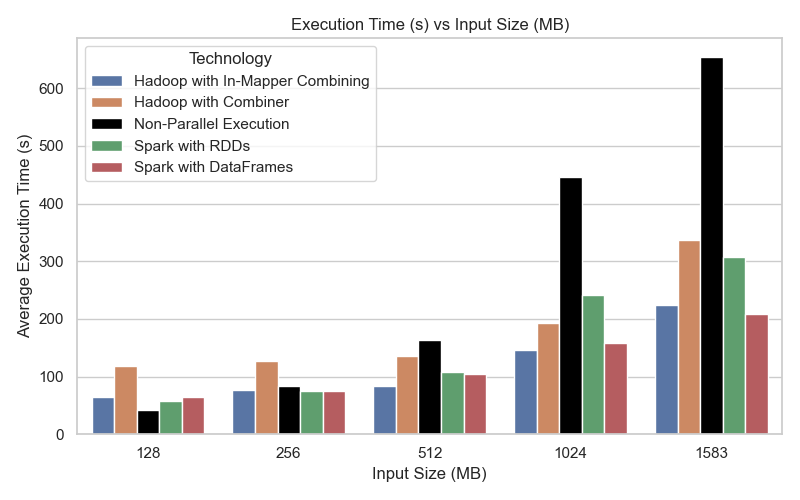
\includegraphics[width=0.444\textwidth]{images/Fig_Execution_Time.png}
	\caption{Execution Time Plot}
	\label{fig:execution-time}
\end{figure}
\begin{figure}[H]
	\centering
	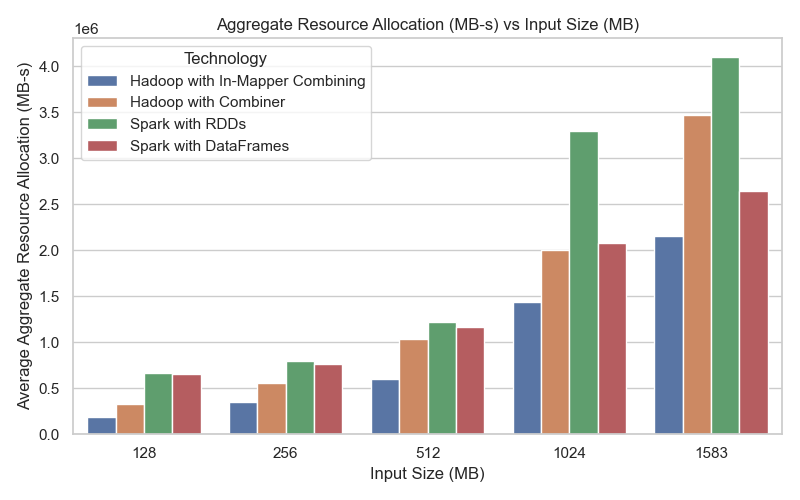
\includegraphics[width=0.444\textwidth]{images/Fig_Aggregate_Resource_Allocation.png}
	\caption{Aggregate Resource Plot}
	\label{fig:aggregate-resource-allocation}
\end{figure}
\begin{figure}[H]
	\centering
	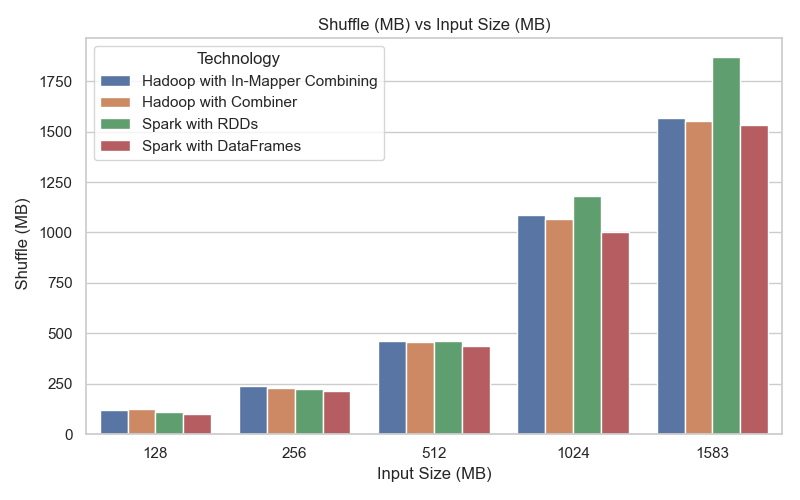
\includegraphics[width=0.444\textwidth]{images/Fig_Shuffle.png}
	\caption{Shuffle Plot}
	\label{fig:shuffle}
\end{figure}

\newpage

\subsection{Effect of Reducers on Performance}

\begin{figure}[H]
	\centering
	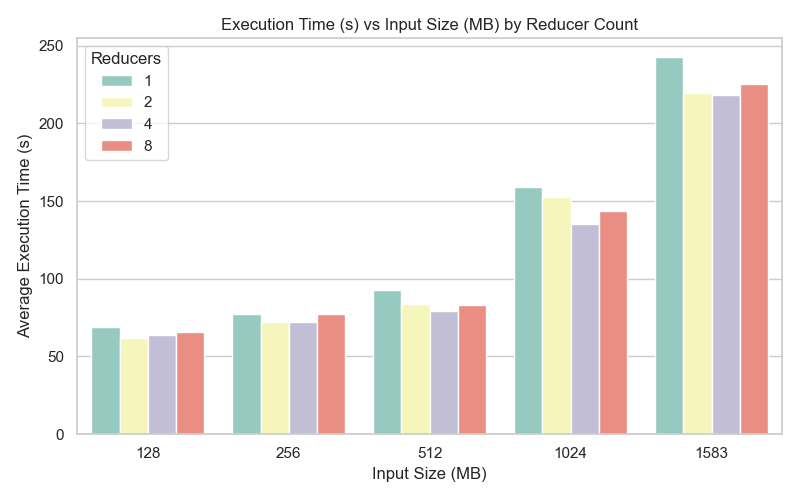
\includegraphics[width=0.5\textwidth]{images/Fig_Reducers_Execution_Time.png}
	\caption{Reducers Execution Time}
	\label{fig:reducer-execution-time}
\end{figure}

\vspace{-5.3mm}

The image above (Fig.~7) shows the impact of varying the number of reducers on the execution time of the Hadoop application.
As input size increases, the difference in performance becomes more pronounced. For small datasets (128MB, 256MB and 512MB), the reducer increase has minimal impact. However, for larger datasets (1024MB and 1583MB), using more reducers generally leads to lower execution times, with the best performance observed when using 4 reducers. It is evident that using a \textbf{single reducer} yields the \textbf{worst performance} across all input sizes. This is likely due to the single reducer becoming a \textbf{bottleneck}, limiting the degree of parallelism and slowing down the entire process. Interestingly, performance slightly degrades when moving from 4 to 8 reducers, likely due to overhead from task coordination and context switching. This suggests that, while increasing reducer count improves parallelism and reduces execution time up to a point, beyond that point the benefits diminish or even reverse. The \texttt{2}- and \texttt{4}-reducer configurations exhibit \textbf{comparable performance} overall. Specifically, the \texttt{2-reducer} setup performs better with \textbf{smaller datasets}, while the \texttt{4-reducer} configuration becomes more efficient as the dataset size increases, likely due to its \textbf{better scalability} with larger workloads.


\begin{figure}[H]
	\centering
	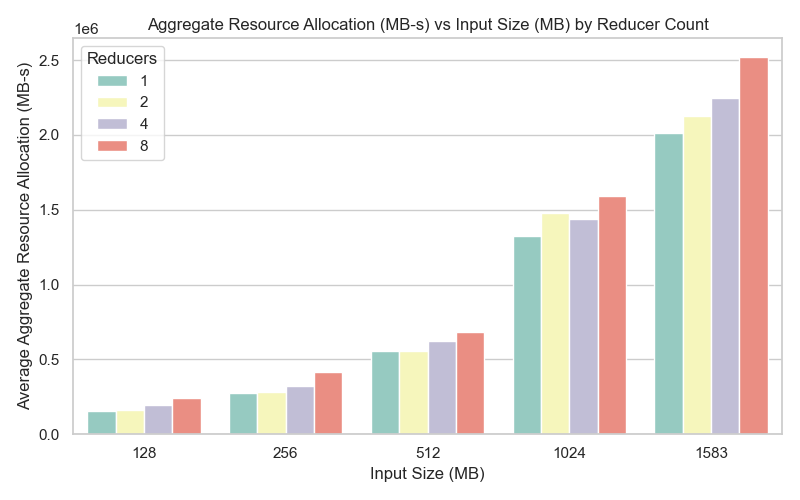
\includegraphics[width=0.5\textwidth]{images/Fig_Reducers_Aggregate_Resource_Allocation.png}
	\caption{Reducers Aggregate Resource Allocation}
	\label{fig:reducer-aggregate-resource-allocation}
\end{figure}

For Aggregate Resource Allocation (Fig.~8), despite some small irregularities in the graph, it is easy to see that there is a pattern: it increases as the number of reducers increases. This behavior is expected, as increasing the number of reducers leads to more concurrent tasks executing in parallel, each requiring its own memory space. As a result, the total memory footprint of the application increases with the number of reducers. Although this allows for better task distribution and reduced execution time, it comes at the cost of higher memory consumption. Therefore, there is a trade-off between parallelism and resource utilization, and selecting the optimal number of reducers involves balancing execution efficiency with memory availability. The only exception occurs at the \texttt{1024MB} input size, likely due to a significant difference in execution time between the \texttt{2-reducer} and \texttt{4-reducer} configurations. 


\subsection{Final Considerations}
The comprehensive evaluation across execution time, memory usage and shuffle volume shows that no single implementation universally dominates every metric, but trade‑offs emerge clearly. \texttt{Hadoop-noimc} suffers from both high CPU time (1154.49\,s) and poor scalability, while \texttt{Spark-RDD} achieves the lowest CPU time (82.59\,s) at the expense of excessive shuffle bytes and aggregate resource allocation (3561005.96\,MB\,$\cdot$\,s on average). \texttt{Hadoop-imc} improves over \texttt{Hadoop-noimc} by reducing both execution time and memory footprint, yet still lags behind the Spark-based approaches for large datasets.

\texttt{Spark with Dataframes} consistently delivers near‑optimal execution times while keeping both aggregate resource allocation (2637719.31\,MB\,$\cdot$\,s) and shuffle volume moderate. This balance of low execution latency, controlled memory consumption and efficient shuffling makes the DataFrame API the best choice for large‑scale word‑count workloads on our cluster. Furthermore, tuning the reducer count to four provides additional speedup in Hadoop jobs, but does not bridge the gap to Spark’s in‑memory processing advantages.

In conclusion, for batch analytics on medium to large datasets, \texttt{Spark with Dataframe} offers the strongest overall performance profile. However, if minimizing memory usage is paramount and data volumes remain moderate, \texttt{Hadoop with In-Mapper Combining} remains a viable alternative.
